\documentclass[crop,tikz]{standalone}

\usepackage{tikz}
\usetikzlibrary{calc, backgrounds, decorations.pathreplacing}

\tikzset{%
	do path picture/.style={%
		path picture={%
			\pgfpointdiff{\pgfpointanchor{path picture bounding box}{south west}}%
			{\pgfpointanchor{path picture bounding box}{north east}}%
			\pgfgetlastxy\x\y%
			\tikzset{x=\x/2,y=\y/2}%
			#1
		}
	},
	sin wave/.style={do path picture={    
			\draw [line cap=round] (-3/4,0)
			sin (-3/8,1/2) cos (0,0) sin (3/8,-1/2) cos (3/4,0);
	}},
	cross/.style={do path picture={    
			\draw [line cap=round] (-2/4,-2/4) -- (2/4,2/4) (-2/4,2/4) -- (2/4,-2/4);
	}},
	plus/.style={do path picture={    
			\draw [line cap=round] (-3/4,0) -- (3/4,0) (0,-3/4) -- (0,3/4);
	}}
}

\tikzset{jump/.style={
		to path={
			let \p1=(\tikztostart),\p2=(\tikztotarget),\n1={atan2(\y2-\y1,\x2-\x1)} in
			(\tikztostart) -- ($($(\tikztostart)!#1!(\tikztotarget)$)!0.15cm!(\tikztostart)$)
			arc[start angle=\n1+180,end angle=\n1,radius=0.1cm] -- (\tikztotarget)}
	},
	jump/.default={0.5}
}

\usepackage{mathtools}
\usepackage{bm}
\usepackage{esvect}


\begin{document}

	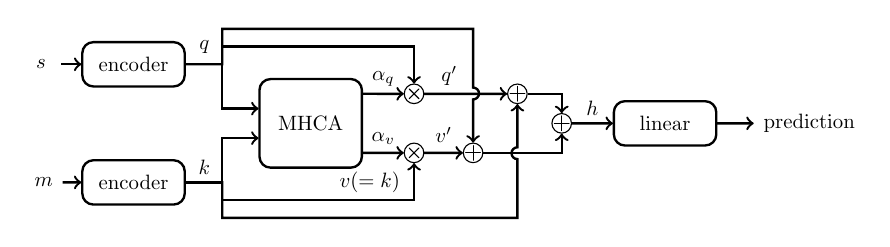
\begin{tikzpicture}[scale=.75, every node/.style={scale=.75}]
	\tikzstyle{sqr} = [rectangle, rounded corners, minimum width=1cm, text width=1.5cm, minimum height=.75cm,text centered, draw=black, line width=.3mm]
	
	\node (m1) [text width=.3cm] {$\vv{{s}}$};
	\node (m2) [text width=.35cm, below of=m1, yshift=-1cm] {$\vv{{m}}$};
	
	\node (enc1) [sqr, right of=m1, xshift=.5cm] {encoder};
	\node (enc2) [sqr, right of=m2, xshift=.5cm] {encoder};
	
	\node (mhca) [sqr, right of=enc1, xshift=2cm, yshift=-1cm, minimum height=1.5cm] {MHCA};
	
	\node (mult1) [circle, draw, cross, right of=mhca, xshift=.75cm, yshift=.5cm] {};
	\node (mult2) [circle, draw, cross, right of=mhca, xshift=.75cm, yshift=-.5cm] {};
	
	\node (p1) [circle, draw, plus, right of=mult1, xshift=.75cm] {};
	\node (p2) [circle, draw, plus, right of=mult2, xshift=-.cm] {};
	
	\node (p3) [circle, draw, plus, right of=p1, xshift=-.25cm, yshift=-.5cm] {};
	
	\node (l1) [sqr, right of=p3, xshift=.75cm] {linear};
	\node (out) [text width=.25cm, right of=l1, xshift=.75cm] {};
	
	\draw[->, line width=.3mm] (m1) -- (enc1);
	\draw[->, line width=.3mm] (m2) -- (enc2);
	\draw[->, line width=.3mm] (enc1) -| +(1.5, -.5) |- ($(mhca.west)+(0, .25)$);
	\draw[->, line width=.3mm] (enc2) -| +(1.5, .5) |- ($(mhca.west)+(0, -.25)$);
	\draw[->, line width=.3mm] ($(mhca.east)+(0, .5)$) -- node [yshift=.25cm] {${\alpha_q}$} (mult1);
	\draw[->, line width=.3mm] ($(mhca.east)+(0, -.5)$) -- node [yshift=.25cm] {${\alpha_v}$} (mult2);
	
	\draw[->, line width=.3mm] (mult1) -- node [yshift=.3cm, xshift=-.28cm] {$\vv{{q'}}$} (p1);
	\draw[->, line width=.3mm] (mult2) -- node [yshift=.3cm, xshift=-.cm] {$\vv{{v'}}$} (p2);
	
	\draw[->, line width=.3mm] (p1) -| (p3);
	\draw[->, line width=.3mm] (p2) -| (p3);
	\draw[->, line width=.3mm] (p3) -- node [yshift=.25cm, xshift=.0cm] {$\vv{{h}}$} (l1);
	\draw[->, line width=.3mm] (l1) -- node [yshift=.0cm, xshift=1.25cm] {prediction} (out);
	
	\node at (5.5, -2) {$\vv{{v}} (=\vv{{k}})$};
	
	\draw[->, line width=.3mm] ($(enc1.east)+(0, .0)$) -| +(.62, .3) -| node [yshift=.0cm, xshift=-3.55cm] {$\vv{{q}}$} (mult1);
	\draw[->, line width=.3mm] ($(enc2.east)+(0, -.0)$)  -| +(.62, -.3) -| node [yshift=.55cm, xshift=-3.55cm] {$\vv{k}$} (mult2);
	\draw[->, line width=.3mm] ($(enc1.east)+(0, .0)$) -| +(.62, .6) -| ($(p2.north)+(0, 1)$) to[jump=0.185] (p2);
	\draw[->, line width=.3mm] ($(enc2.east)+(0, -.0)$) -| +(.62, -.6)  -| ($(p1.south)+(0, -1)$) to[jump=0.185] (p1);
	
	\end{tikzpicture}

\end{document}